\chapter{Griegas por pesos de Malliavin}\label{cap:griegas}

Sea $V(\theta)=\E[e^{-rT}\Phi(S_T^\theta)]$. Las diferencias finitas tienen sesgo
$O(h^2)$ y varianza $O(h^{-2})$ (o $O(h^{-3})$ para la gamma) si $\Phi$ es
discontinua; el método \emph{pathwise} exige $\Phi$ diferenciable. Aplicando
\eqref{eq:peso} \cite{fournie1999}:
\[
  \partial_\theta V=\E\big[e^{-rT}\Phi(S_T)\,\pi_\theta\big],
\]
con pesos que no dependen de $\Phi$. En el modelo de Black--Scholes:
\begin{align*}
  \pi_\Delta&=\frac{W_T}{S_0\sigma T}, &
  \pi_{\mathcal V}&=\frac{W_T^2}{\sigma T}-W_T-\frac1\sigma,\\
  \pi_\Gamma&=\frac{\pi_{\mathcal V}}{S_0^2\sigma T}, &
  \pi_\rho&=\frac{W_T}{\sigma}-T.
\end{align*}

\paragraph{Derivación de $\pi_\Delta$.} $\partial_{S_0}V=e^{-rT}\E[\Phi'(S_T)S_T/S_0]$ y
$\ip{\D S_T}{\ind}=\sigma S_TT$. Con $u=\ind$ y $G=S_T/S_0$ en \eqref{eq:peso}:
$\dive\big(\tfrac{1}{S_0\sigma T}\big)=\tfrac{W_T}{S_0\sigma T}$.

\section{Opción asiática}
Sea $A=\frac1T\int_0^TS_t\dd t$. Con $u_t=S_t$:
$\ip{\D A}{u}=\tfrac{\sigma}{T}\int_0^TS_s\int_s^TS_t\dd t\dd s=\tfrac{\sigma T}{2}A^2$, y
\[
  \Delta=\frac{e^{-rT}}{S_0}\E\Big[\Phi(A)\Big(\frac{2(S_T-S_0)}{\sigma^2TA}-\frac{2r}{\sigma^2}+1\Big)\Big].
\]

\begin{observacion}
Para pagos suaves (call) el estimador de Malliavin puede tener \emph{más} varianza
que el pathwise; las técnicas de localización y pesos óptimos
\cite{fournie2001,benhamou2003} combinan lo mejor de ambos.
\end{observacion}

\begin{figure}[h]
  \centering
  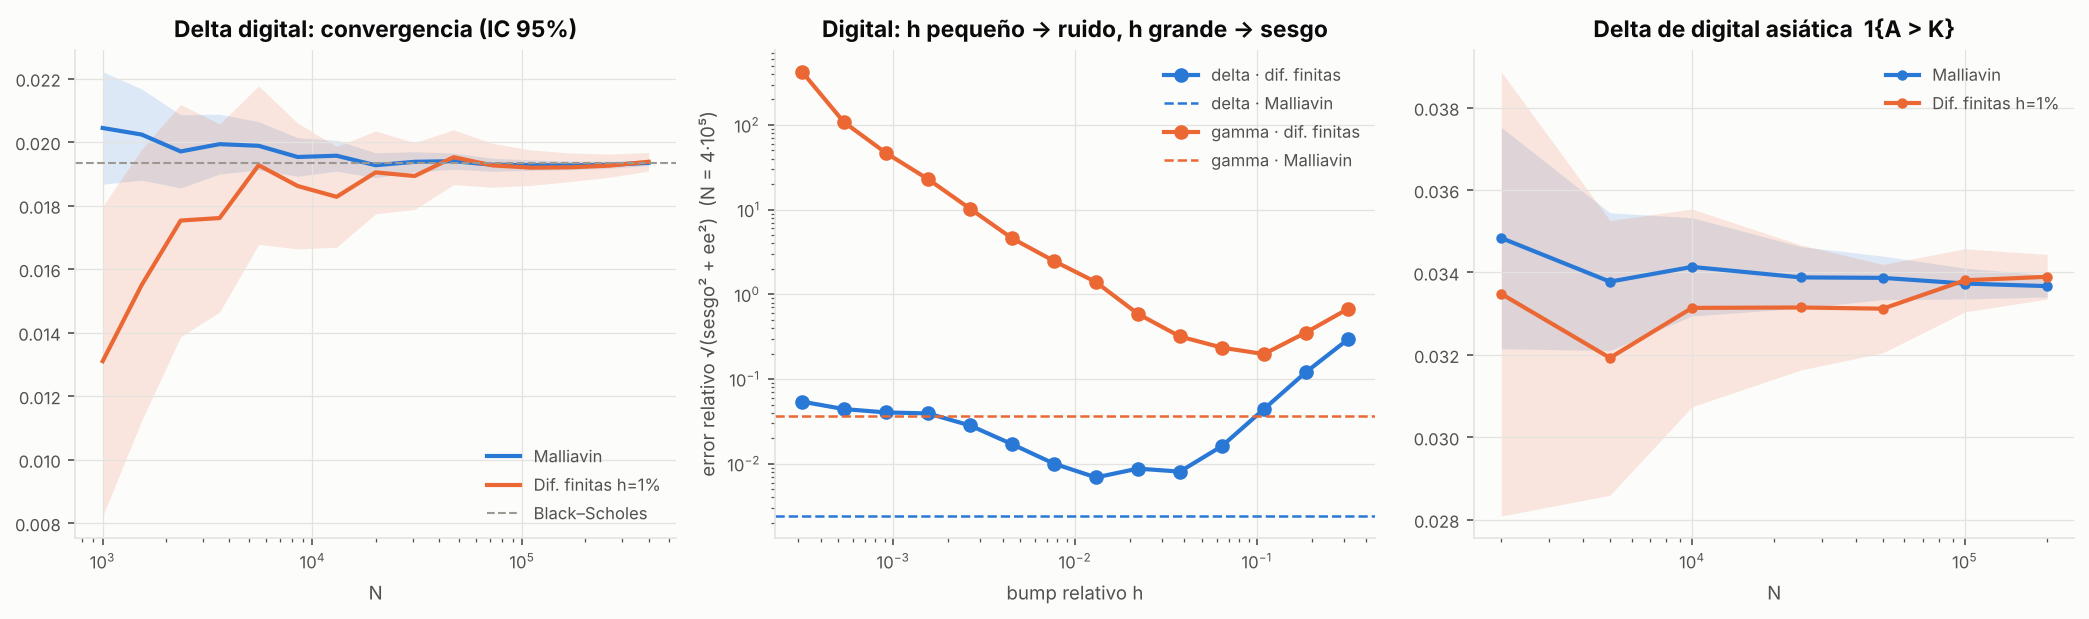
\includegraphics[width=\linewidth]{05_griegas_malliavin}
  \caption{Delta digital, compromiso sesgo--varianza en $h$, y delta de una digital
  asiática (\codigo{examples/05\_griegas\_malliavin.py}).}
\end{figure}
